First, we need to measure precisely how the engines respond to any arbitrary input, to design they're own control loop.
To measure the servo response, we proceeded in two times : A first session, with some electronic specialized tool, 
and a second session with the MCU as controller and measuring unit !

\paragraph{}
We used this schematic for the measures :
\begin{figure}[!hbt]
    \centering
    \resizebox{\SchematicWidth}{!}{%
        \begin{circuitikz}
            % ---------------------------------------------------------------------------
            % Draw components
            % ---------------------------------------------------------------------------
            \draw (0,0) node[ground] {} to[vsourcesquare, label=\(V_{\text{PWM}}\)] (0,2) node[] () {};
            \draw (4,2) node[elmech](motor){M};
            \draw (4,0) node[ground] {};
            \draw (4,4) node[vcc] {\(V_{\text{CC}} = 5 \si{\volt}\)};
            \draw (8,2) node[oscopeshape] (osc1) {};
            \draw (2,1) node[oscopeshape] (osc2) {};

            % ---------------------------------------------------------------------------
            % Draw wires
            % ---------------------------------------------------------------------------
            \draw (0,2) -- (motor.left);
            \draw (4,0) -- (motor.bottom);
            \draw (4,4) -- (motor.top);
            \draw (motor.right) -- (osc1.left);
            \draw (osc2.left) -- ++(-0.5, 0) -- ++(0,1) node[circ] {};

        \end{circuitikz}}

    \caption{Schematic used for testing response of servo engines}
    \label{fig:Servo_test}
\end{figure}

\paragraph{}
For the first session, we sent the control signal using a dedicated signal generator, configured 
to output a PWM at a frequency of $50 \si{\hertz}$ and with a pulse length between $1 \si{ms}$ and
$2 \si{ms}$.
We measured the output of the servo engines, which is an analog output that reflect the servo position
using an oscilloscope.

\begin{figure}[!hbt]
    \centering
    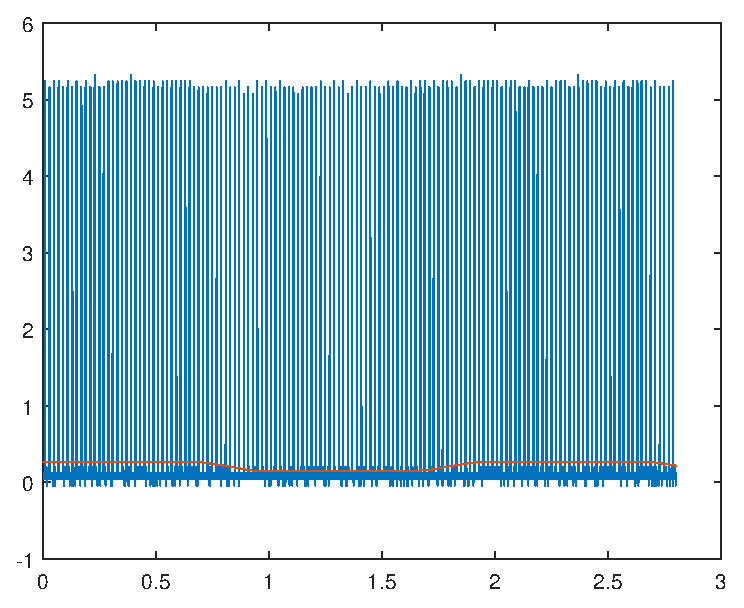
\includegraphics[width=\SchematicWidth]{\Images/Servos/time-domain-response.eps}
    \caption{Time domain servo response}
\end{figure}
\FloatBarrier

\paragraph{}
We can see on this image... nothing ! That's because the pulse length if near 0 compared to the whole
period. And even then, the servo response is quite slow, thus we need a long measure time !

To exploit this data, we used the Matlab "DutyCycle" function, that return the actual duty cycle of a signal.
This gave us results that where ok, but clearly perfectibles :

\begin{figure}[!hbt]
    \centering
    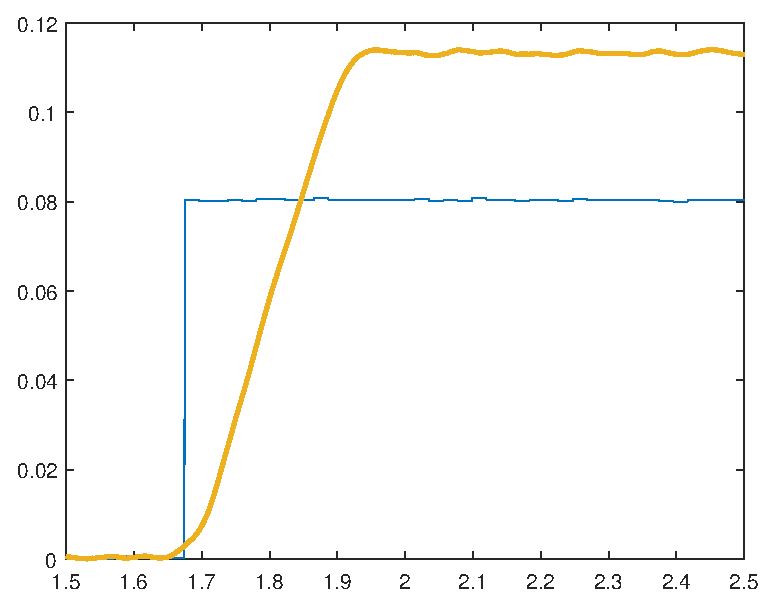
\includegraphics[width=\SchematicWidth]{\Images/Servos/Duty-Forced.eps}
    \caption{Time domain servo response, expressed in duty cycle}
\end{figure}
\FloatBarrier

\paragraph{}
Now, we have a command and a response that seem plausible, except one details : The servo seems to start 
\textit{before} the command. That's typically the case for a non-causal systems, which can't be easily controlled,
if at all !
Luckily, in our case this is an issue from the code that draw theses graphes, rathers than the servo by itself.
We used a script that convert the raw measures to theses ones, but there was a bug, which cause this lag \footnote{
    To be precise, the DutyCycle function return a list of n elements, where n is the number of period. We then
    extended this list to match the original lenght. And since the DutyCycle return the value at the end of the 
    period, there is $Te$ retard. Thus, a $\frac{1}{Te}$ period is now $\frac{n}{Te}$. 
    Combine both, and you end up with a visually non-causal system.
}.

\paragraph{}
Anyway, theses measures weren't that good, they gave a first order approximation but didn't represented 
correctly the signal. This was caused by multiple points :

\begin{itemize}
    \item Error on the signal generator : When working at this kind of low frequencies, the signal is quite imprecise.
    \item Too big amplitude on the command. This lead to results that are outisde the interresting range.
\end{itemize}

\paragraph{}
We addressed most of theses points on the second session of measure, where we used the final MCU to control the servos.
We thus got a precise (Up to $\pm 1 \si{\mu\second}$) pulses, and the definitive measure device (the integrated ADC)\footnote{
    Which was already characterized at this point, but, for clarity reasons is explicited in the next section
}.

We got theses measures :

\begin{figure}[!hbt]
    \centering
    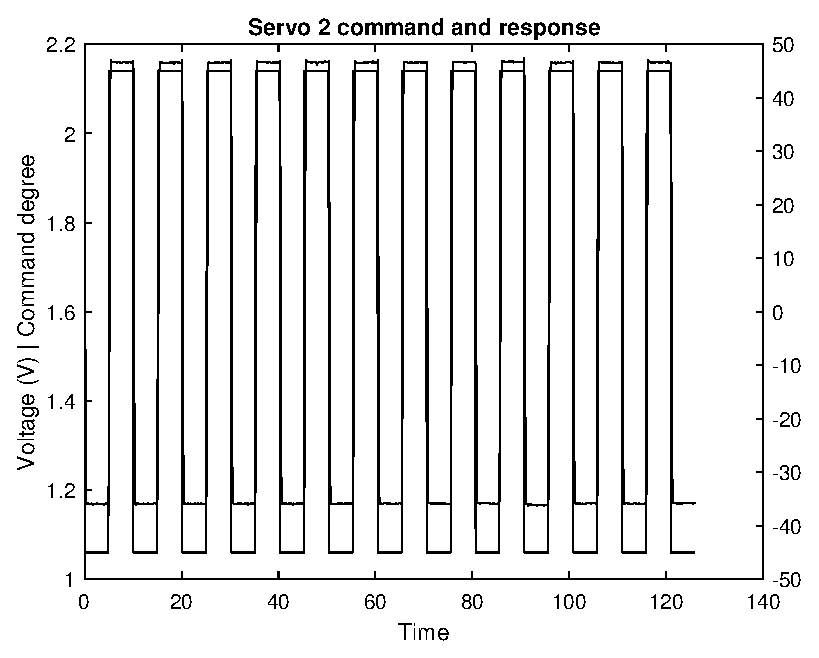
\includegraphics[width=\SchematicWidth]{\Images/Servos/reduced-square.eps}
    \caption{Time domain servo response, expressed in duty cycle}
\end{figure}
\begin{figure}[!hbt]
    \centering
    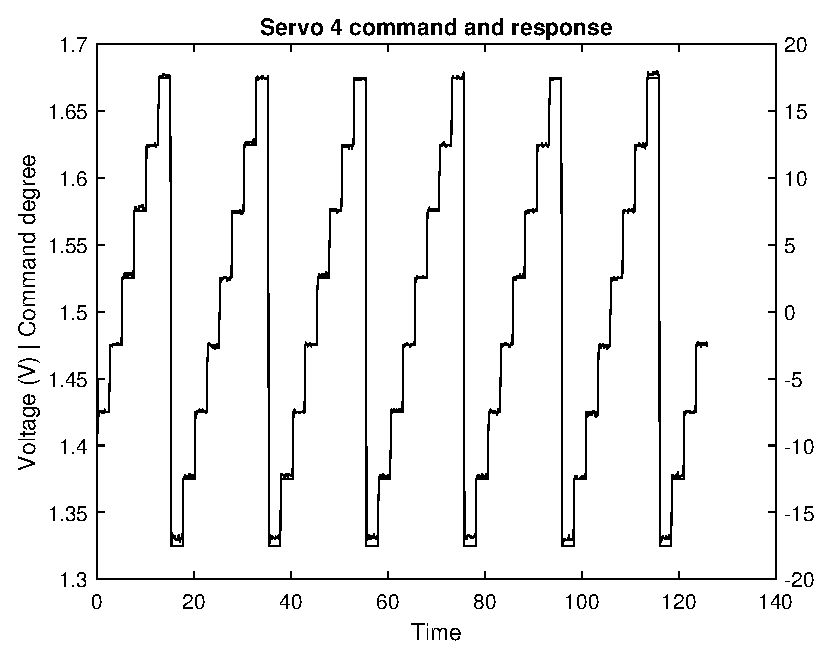
\includegraphics[width=\SchematicWidth]{\Images/Servos/ramp.eps}
    \caption{Time domain servo response, expressed in duty cycle}
\end{figure}
\FloatBarrier

\paragraph{}
Theses are way better than we got on the first session, because we addresses the issues.

Using the zoom functions, we can identify that in our case, the servos engines are responsing
as a very simple device : A first order one.

They goes into the required position in about $1 Te$, which is on our system arround 
$120 \si{\milli\second}$ by achieving a linear transition.


